\documentclass[]{../template/Report}%方括号内写yuxi即生成预习报告\documentclass[yuxi]{../template/Report}
\settemplatedir{../template/}%设置模板路径

\exname{密立根油滴实验} %实验名称
\extable{} %实验桌号
\instructor{} %指导教师
\class{} %班级
\name{} %姓名
\stuid{} %学号

\nyear{} %年
\nmonth{} %月
\nday{} %日
\nweekday{} %星期几,e.g. \nweekday{三}
\daypart{}%上午/下午,e.g. \daypart{上}

\redate{} %如有实验补做,补做日期
\resitu{} %情况说明:

\begin{document}
\makecover%输出封面

\section{预习报告(10分)}

\subsection{实验综述(5分)}
\subsubsection{实验现象}
\begin{enumerate}
    \item 平行板不加电压时,油滴因重力加速下降,受空气黏滞阻力后匀速;
    \item 加电压使油滴所受重力与静电力平衡,油滴静止;
    \item 改变油滴电荷,平衡电压呈特定值变化。
\end{enumerate}
\subsubsection{实验原理及方法}
\textbf{基本实验原理:}采用静态平衡法。如下图,利用密立根油滴仪将油滴喷入两块相距为$d$的水平放置的平行带电平板之间,油滴由于摩擦一般带电,设油滴质量为$m$,带电量$q$,两极电压为$U$,油滴受重力和静电力动态平衡满足$mg = qE = q\frac{U}{d}$
\begin{figure}[!h]
    \begin{center}
        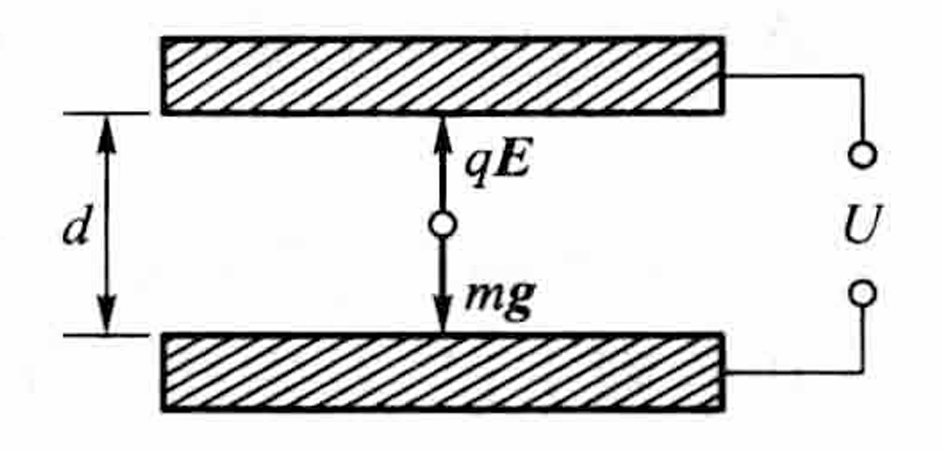
\includegraphics[width=0.5\textwidth]{figues/limigen/yuanli.png}
        \caption{基本实验原理图}
    \end{center}
\end{figure}

\textbf{油滴质量的测定:}设小球状的油滴密度为$\rho$,半径为$r$,则质量$m = \frac{4}{3}\pi r^3\rho$。在平行板不加电压时,油滴受重力加速下降,油滴达到某一速度后阻力与重力平衡时匀速下降满足斯托克斯定律修正公式:
\[ F = \frac{6\pi r\eta v}{1 + \frac{b}{pr}} \]
根据修正后的黏滞阻力公式,得油滴半径:
\[ r = \sqrt{\frac{9\eta}{2\rho g}} \cdot \frac{1}{\sqrt{1 + \frac{b}{pr}}} \]

\textbf{油滴匀速下降速度$v$的测定:}在平行板未加电压时,测出下降长度$l$所用时间$t$,则$v = \frac{l}{t}$

\vspace{2mm}
\textbf{油滴电荷量及基本电荷量:}综合上述公式,得油滴电荷量:
\[ q = \frac{18\pi}{\sqrt{2\rho g}} \left( \frac{\eta l}{t\left(1 + \frac{b}{pr}\right)} \right)^{\frac{3}{2}} \cdot \frac{d}{U} \]
改变油滴的电荷量$q$,使其能达到平衡的电压$U$都取某些特定值$U_n$,它们都满足\(q = m g\frac{d}{U_n} = n e\),式中\(n = \pm1,\pm2,\cdots\),而$e$则是一个不变的值,证明了电荷的不连续性,且\(e = \frac{q}{n}\)。

\vspace{2mm}
\textbf{“逐次相减法” 求基本电荷量:}对n个油滴的电荷量值做逐次相减,估计基本电荷,确定各个油滴的基本电荷数$n$,然后用\(e_i = \frac{q_i}{n}\)公式求算出各个油滴的基本电荷量,取平均值得到$e$。

\subsection{实验重点(3分)}
\begin{enumerate}
    \item 需掌握油滴受力平衡条件,明确重力、静电力、空气黏滞阻力的作用关系,以及电荷量子化的推导逻辑,这是实验数据处理和结果分析的基础;
    \item 测定电子的基本电荷量$e$;
    \item 通过\(e = \frac{q}{n}\)验证电荷的不连续性。
\end{enumerate}

\subsection{实验难点(2分)}
\begin{enumerate}
    \item 难以快速筛选出符合要求的油滴,过大的油滴下降过快,时间测量误差大;过小的油滴易受气流干扰,难以稳定跟踪;
    \item 通过微调电压,确保油滴在 10-20 秒内位置无明显变化,避免因电压调节过度或不足导致误判平衡状态;
    \item 需排除多种干扰因素,如极板电压波动、空气对流等。
\end{enumerate}

\begin{fullreportonly}
\section{原始数据(20分)}
\begin{figure}[!h]
    \begin{center}
        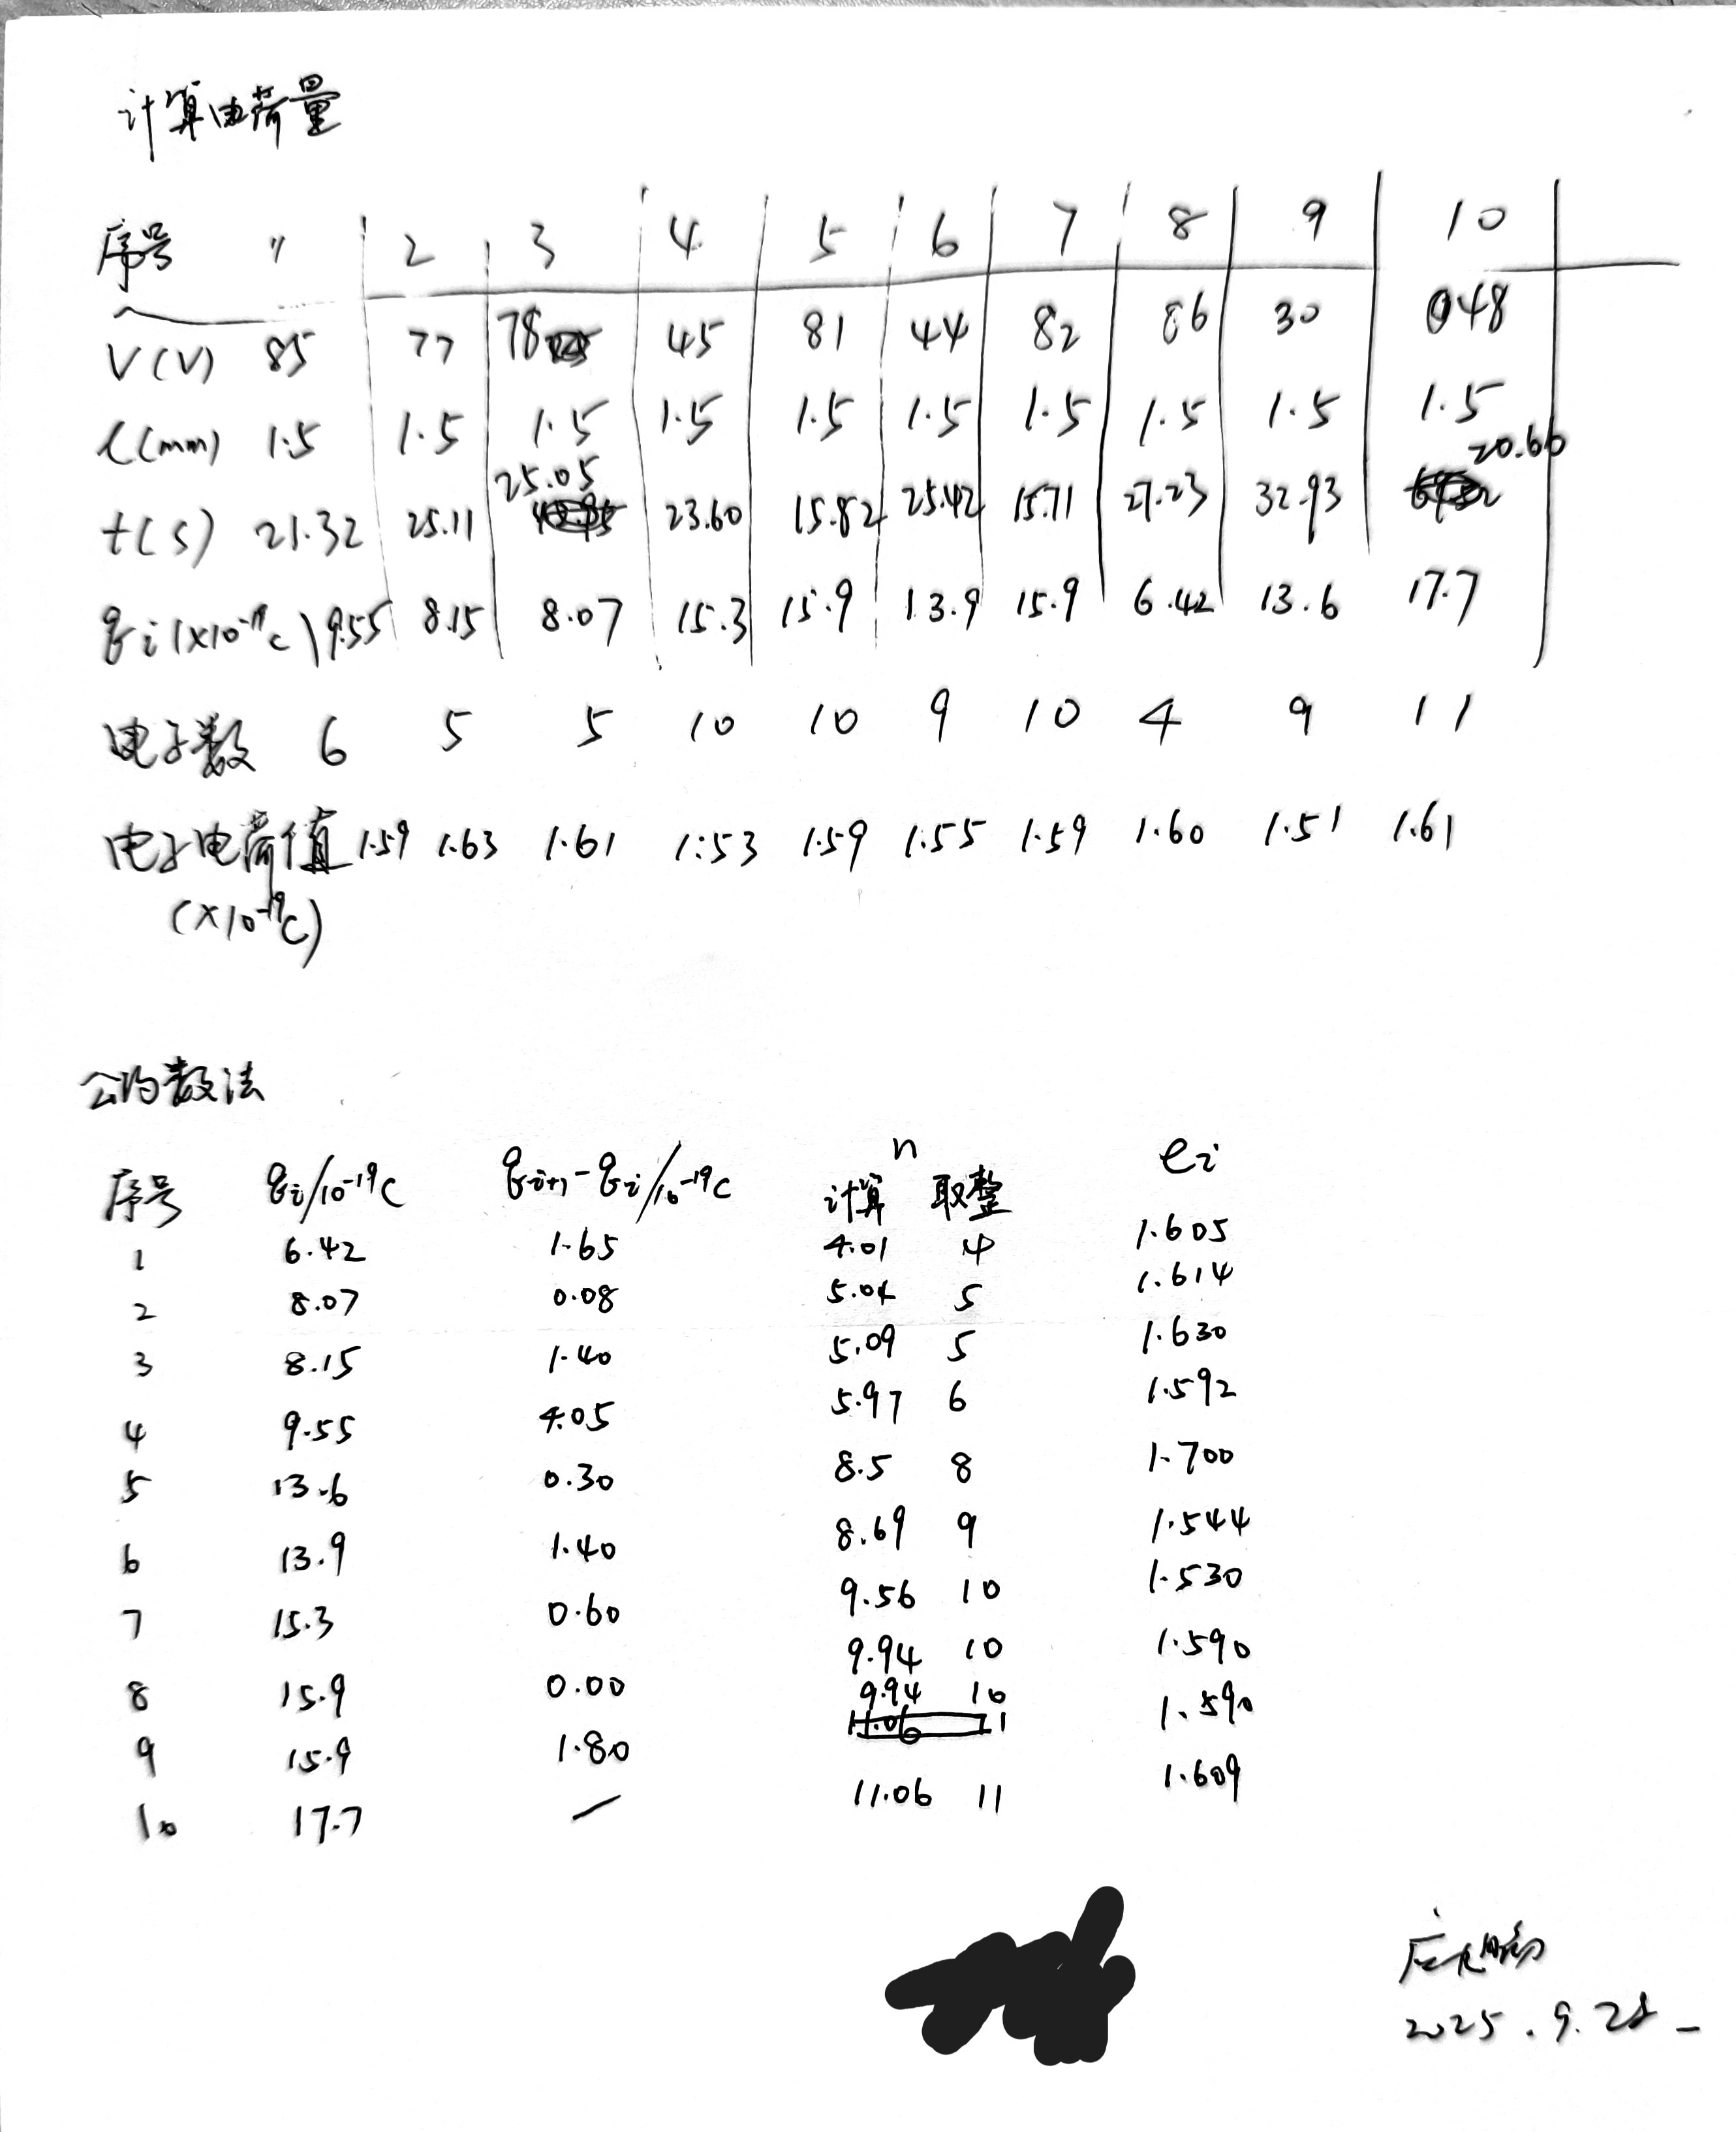
\includegraphics[width=0.4\textwidth]{exp_data/miligen.jpg}
        \caption{原始数据}
    \end{center}
\end{figure}

\section{结果与分析(60分)}
\subsection{数据处理与结果(30分)}
\subsubsection{测量与计算结果}
经过多次测量,记录平衡电压$V$,将开关拨到“0V”挡,选择一段运动计时,记录计时器读数$t$以及下降距离$l$,再应用上述公式:
\[ q = \frac{18\pi}{\sqrt{2\rho g}} \left( \frac{\eta l}{t\left(1 + \frac{b}{pr}\right)} \right)^{\frac{3}{2}} \cdot \frac{d}{U} \]
计算出油滴带电量,得到下表:
\begin{table}[htbp]
  \centering
  \caption{测量所得$V,l,t$及计算所得电荷量$q$}
  \begin{tabular}{@{}ccccccccccc@{}}
    \toprule
    序号 & 1 & 2 & 3 & 4 & 5 & 6 & 7 & 8 & 9 & 10 \\
    \midrule
    \( V(V) \) & 85 & 77 & 78 & 45 & 81 & 44 & 82 & 86 & 30 & 48 \\
    \( l(mm) \) & 1.5 & 1.5 & 1.5 & 1.5 & 1.5 & 1.5 & 1.5 & 1.5 & 1.5 & 1.5 \\
    \( t(s) \) & 21.32 & 25.11 & 25.05 & 23.60 & 15.82 & 25.42 & 15.71 & 21.23 & 32.93 & 20.66 \\
    \( q_i(\times10^{-19}C) \) & 9.55 & 8.15 & 8.07 & 15.3 & 15.9 & 13.9 & 15.9 & 6.42 & 13.6 & 17.7 \\
    \bottomrule
  \end{tabular}
\end{table}

\subsubsection{公约数法计算基本电荷量}
将上述数据中的电荷量升序排列并逐次相减,从而确定各个油滴的基本电荷数$n$,再用$e_i=\frac{q_i}{n}$求得当前油滴的基本电荷量,如下表:
\begin{table}[htbp]
  \centering
  \caption{公约数法计算基本电荷量}
    \begin{tabular}{@{\hspace{1em}}cccccc@{\hspace{1em}}}
    \toprule
    序号 & \( q_i/10^{-19}\text{C} \) & \( q_{i+1}-q_i/10^{-19}\text{C} \) & \( n \)(计算)& \( n \)(取整) & \( e_i \) \\
    \midrule
    1 & 6.42 & 1.65 & 4.01 & 4 & 1.605 \\
    2 & 8.07 & 0.08 & 5.04 & 5 & 1.614 \\
    3 & 8.15 & 1.40 & 5.09 & 5 & 1.630 \\
    4 & 9.55 & 1.05 & 5.97 & 6 & 1.592 \\
    5 & 13.6 & 0.30 & 8.5 & 8 & 1.700 \\
    6 & 13.9 & 1.40 & 8.69 & 9 & 1.544 \\
    7 & 15.3 & 0.60 & 9.56 & 10 & 1.530 \\
    8 & 15.9 & 0.00 & 9.94 & 10 & 1.590 \\
    9 & 15.9 & 1.80 & 10.06 & 11 & 1.590 \\
    10 & 17.7 & — & 11.06 & 11 & 1.609 \\
    \bottomrule
  \end{tabular}
\end{table}
\clearpage
\subsubsection{求相对误差与A类不确定度}
电子电荷的公认值为:\(e_标 = 1.602 \times 10^{-19} \, \text{C}\)

\vspace{2mm}
\textbf{计算测量值的算术平均值\(\bar{e}\):}计算上述数据平均值最终得到
\[\bar{e}=\frac{\sum_{n = 1}^{10}e_i}{10}\approx 1.589 \times 10^{-19} \, \text{C}\]

\textbf{计算相对误差:}将$e_标与\bar{e}$代入相对误差公式:
\[\text{相对误差} = \left| \frac{\bar{e} - e_{\text{标准}}}{e_{\text{标准}}} \right| \times 100\%\]
得到
\[\text{相对误差} = \left| \frac{1.589 - 1.602}{1.602} \right| \times 100\% \approx 0.79\%\]

\vspace{2mm}
\textbf{计算A类不确定度:}A类不确定度公式采用贝塞尔公式,自由度 \( \nu = n-1 = 9 \):
\[u_A = \sqrt{\frac{1}{n(n-1)} \sum_{i=1}^n (e_i - \bar{e})^2}\]
代入得$u_A \approx 0.013 \times 10^{-19} \, \text{C}$

\vspace{2mm}
最终测量结果可表示为:\(e = (1.589 \pm 0.013) \times 10^{-19} \, \text{C} \quad (\text{相对误差} \approx 0.79\%)\)
\subsection{误差分析(20分)}
\begin{enumerate}
    \item 油滴在实验过程中会逐渐挥发,质量和带电量发生变化,使油滴实际处于动态平衡,难以精准判断静态平衡状态,影响平衡电压的测量;
    \item 油滴并非严格的匀速直线运动,空气阻力与速度的关系及油滴的变速运动过程,会导致下落时间测量存在误差;
    \item 由于人眼观察的局限性,难以精准判断油滴是否完全静止,平衡电压的取值存在误差;
    \item 实验中的空气密度、粘滞系数、重力加速度、大气压等环境参数会随实验条件变化,影响油滴质量、阻力等相关计算。
\end{enumerate}

\subsection{实验探讨(10分)}
在实验操作层面,这是一个对操作技巧要求较高的实验。从喷雾器的使用,到在显微镜下寻找合适的油滴,再到精准调节平衡电压以及测量油滴下落时间,每一个步骤都需要耐心与细心。

\vspace{2mm}
在对实验原理的理解上,我有了更深入的认识。通过实际操作,我更清晰地明白了各个物理量之间的关联,以及公式推导过程中近似处理的意义。

\vspace{2mm}
在数据处理方面,我接触到了 “逐差相减” 等数据处理方法,掌握了一种新的、实用的数据处理思路。

\section{思考题(10分)}
\subsection{在测量油滴匀速下降一段距离$l$所得时间$t$时,应选择哪段$l$最合适?为什么?}
应选择油滴匀速下落阶段的中间一段距离$l$最合适。因为油滴从静止开始下落时,会先经历加速过程,只有当空气粘滞阻力与重力平衡后,才会做匀速直线运动。选择匀速阶段的中间段距离测量时间,能最大程度保证油滴处于匀速运动状态,从而使测量的时间$t$更准确,减小因油滴非匀速运动带来的误差。
\subsection{何谓合适的待测油滴?如何选择?}
合适的待测油滴是大小适中、亮度合适且运动相对稳定的油滴。

\vspace{2mm}
选择方法为:在显微镜下观察,一般选择那些在视野中清晰可见、运动时相对平稳,既不会快速消失,也不会因布朗运动过于剧烈而难以跟踪的油滴。
\subsection{对油滴进行跟踪测量时,有时油滴逐渐变得模糊,为什么?应如何避免在测量途中丢失油滴?}
因为油滴在实验过程中会挥发,质量减小,同时可能受到环境气流等因素影响,导致其与显微镜的对焦状态改变。

\vspace{2mm}
为避免在测量途中丢失油滴,应:
\begin{enumerate}
    \item 尽量选择质量相对较大、挥发较慢的油滴;
    \item 操作时动作轻柔,减少气流扰动;
    \item 密切跟踪油滴的运动,及时微调显微镜焦距,保持油滴始终处于清晰的观察视野中。
\end{enumerate}
\end{fullreportonly}
\insertnotes
\end{document}